\begin{frame}

\begin{center}
\begin{tabular}{c c c}

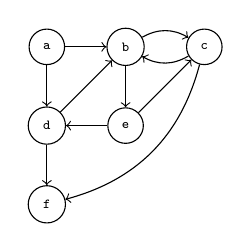
\begin{tikzpicture}[]
\node[draw, circle] (a) at (0, 0) {\tiny \texttt{a}};
\node[draw, circle] (b) at (1, 0) {\tiny \texttt{b}};
\node[draw, circle] (c) at (2, 0) {\tiny \texttt{c}};
\node[draw, circle] (e) at (1, -1) {\tiny \texttt{e}};
\node[draw, circle] (f) at (0, -2) {\tiny \texttt{f}};
\node[draw, circle] (d) at (0, -1) {\tiny \texttt{d}};

\draw[->] (a) -- (b);
\draw[->] (b) edge[bend left] (c);
\draw[->] (b) -- (e);
\draw[->] (c) edge[bend left] (f);
\draw[->] (e) -- (d);


\draw[->] (c) edge[bend left] (b);
\draw[->] (d) edge[] (b);

\draw[->] (a) edge[] (d);
\draw[->] (e) edge[] (c);
\draw[->] (d) edge[] (f);
\end{tikzpicture}

&

\quad

&

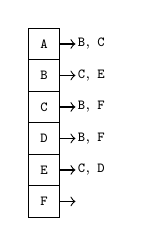
\begin{tikzpicture}[scale = 0.4]
\draw (0, 0) grid (1, 6);
\node at (0.5, 0.5) {\tiny \texttt{F}};
\node at (0.5, 1.5) {\tiny \texttt{E}};
\node at (0.5, 2.5) {\tiny \texttt{D}};
\node at (0.5, 3.5) {\tiny \texttt{C}};
\node at (0.5, 4.5) {\tiny \texttt{B}};
\node at (0.5, 5.5) {\tiny \texttt{A}};

\draw[->] (1, 0.5) -- (1.5, 0.5);
\draw[->] (1, 1.5) -- (1.5, 1.5);
\draw[->] (1, 2.5) -- (1.5, 2.5);
\draw[->] (1, 3.5) -- (1.5, 3.5);
\draw[->] (1, 4.5) -- (1.5, 4.5);
\draw[->] (1, 5.5) -- (1.5, 5.5);


\node at (2, 5.5) {\tiny \texttt{B}, \texttt{C}};
\node at (2, 4.5) {\tiny \texttt{C}, \texttt{E}};
\node at (2, 3.5) {\tiny \texttt{B}, \texttt{F}};
\node at (2, 2.5) {\tiny \texttt{B}, \texttt{F}};
\node at (2, 1.5) {\tiny \texttt{C}, \texttt{D}};
\end{tikzpicture}

\end{tabular}
\end{center}

DFS execution from node \texttt{a}

\begin{center}
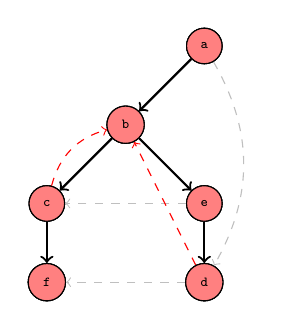
\begin{tikzpicture}[]

\node[draw, circle] (a) at (0, 0) {\tiny \texttt{a}};

\pause

\node[draw, fill = green!50!white, circle] (a) at (0, 0) {\tiny \texttt{a}};

\pause

\node[draw, circle] (b) at (-1, -1) {\tiny \texttt{b}};
\draw[->, thick] (a) -- (b);

\pause

\node[draw, fill = green!50!white, circle] (b) at (-1, -1) {\tiny \texttt{b}};

\pause

\node[draw, circle] (c) at (-2, -2) {\tiny \texttt{c}};
\draw[->, thick] (b) -- (c);

\pause 

\node[draw, fill = green!50!white, circle] (c) at (-2, -2) {\tiny \texttt{c}};

\pause

\draw[->, dashed, red] (c) edge[bend left] (b);

\pause

\node[draw, circle] (f) at (-2, -3) {\tiny \texttt{f}};
\draw[->, thick] (c) -- (f);

\pause

\node[draw, fill = green!50!white, circle] (f) at (-2, -3) {\tiny \texttt{f}};

\pause

\node[draw, fill = red!50!white, circle] (f) at (-2, -3) {\tiny \texttt{f}};

\pause

\node[draw, fill = red!50!white, circle] (c) at (-2, -2) {\tiny \texttt{c}};

\pause

\node[draw, circle] (e) at (0, -2) {\tiny \texttt{e}};
\draw[->, thick] (b) -- (e);

\pause

\node[draw, fill = green!50!white, circle] (e) at (0, -2) {\tiny \texttt{e}};

\pause

\draw[->, dashed, gray!50!white] (e) edge[] (c);

\pause

\node[draw, circle] (d) at (0, -3) {\tiny \texttt{d}};
\draw[->, thick] (e) -- (d);

\pause

\node[draw, fill = green!50!white, circle] (d) at (0, -3) {\tiny \texttt{d}};

\pause

\draw[->, dashed, red] (d) edge[] (b);

\pause 

\draw[->, dashed, gray!50!white] (d) edge[] (f);

\pause

\node[draw, fill = red!50!white, circle] (d) at (0, -3) {\tiny \texttt{d}};

\pause

\node[draw, fill = red!50!white, circle] (e) at (0, -2) {\tiny \texttt{e}};

\pause

\node[draw, fill = red!50!white, circle] (b) at (-1, -1) {\tiny \texttt{b}};

\pause

\draw[->, dashed, gray!50!white] (a) edge[bend left] (d);

\pause


\node[draw, fill = red!50!white, circle] (a) at (0, 0) {\tiny \texttt{a}};



\end{tikzpicture}
\end{center}

\end{frame}